
\section{Bandwidth-Aware Segmented Gossip Aggregation}

Now consider the network topology with $n$ workers. An all-reduce worker pushes $n-1$ local model replicates to the other workers through $n-1$ links while a gossip worker is expected to push one local model replicate out through only one link. Within a datacenter where the workers are connected by the local area network, they can always communicate with each other at maximum bandwidth thus the gossip worker can achieve great speed up as the transmission size is drastically reduced.

However, in the federated learning context where the workers are geo-distributed, the real bandwidth between the workers is typically small due to the potential bottleneck of WAN. Thus the traditional gossip-based schemes can not make full use of the worker's bandwidth because the transmissions are limited in one or few links. We propose the \emph{Segmented Gossip Aggregation} to solve this problem by "splitting" the transmission task and feeding them into more links.

%In the \sys solution, the worker takes the responsibility of data flow: to communicate actively the local model with a portion of peers, transfer local model and aggregate local model. The intuition of \textit{Active} borrows the idea from Gossip-based protocols in which the workers actively push the models to peers. By doing this, the heavy traffic in $n$ links of parameter server could be dissolved among the $n(n-1)$ links between $n$ workers.
%

\subsubsection{Segmented Pulling}

Fig. \ref{Fig: Segment sub.1} illustrates the transfer procedure with segmented gossip aggregation which we name it \emph{segmented pulling.} In the aggregation phase, the worker needs to receive the model parameters from others. While the naive gossip-based synchronization schemes require the worker to collect the whole model parameters, segmented pulling allows the worker to pull different parts of the model parameters from different workers and rebuild a mixed model for aggregation.

Let $\mathcal{W}$ denote the model parameters. The worker firstly breaks the structure of $\mathcal{W}$ into $S$ segments without overlapping such that
\begin{equation}
    \mathcal{W} = (\mathcal{W}[1],\mathcal{W}[2],\dots,\mathcal{W}[S])
\end{equation}

For each segment $l$, the worker chooses a peer worker which we denote it as $j_l$ and then actively pulls the corresponding segment $\mathcal{W}_{j_l}[l]$ from it. Note that this step is parallelized to make full use of the bandwidth. When the worker fetches all the model segments back, a new mixed model $\mathcal{W}^\prime$ can be rebuilt from the segments such that
\begin{equation}
    \mathcal{W}^\prime = (\mathcal{W}_{j_1}[1],\mathcal{W}_{j_2}[2],\dots,\mathcal{W}_{j_l}[S])
\end{equation}

The naive gossip-based scheme pulls all the segments from a single peer worker. However, with segmented pulling, if we choose a different peer for each segment, the total transmission size is still equal to one model, like the naive gossip-based schemes, but the traffic is dissolved among not one but $S$ links.


\subsubsection{Bandwidth-Aware Worker Selection}
The WAN bandwidth not only varies significantly between different regions (e.g., up to $12 \times$ of bandwidth variance between geographically-close regions and distant regions), but also is time-varying (e.g., up to $10 \times$ of bandwidth variance within a day), as shown by other systems \ref{}.  Thus, to reduce the transmission time, we tend to select 

Taking the advantage of epsilon-greedy, we 


%\begin{figure}[H]
%\centering 
%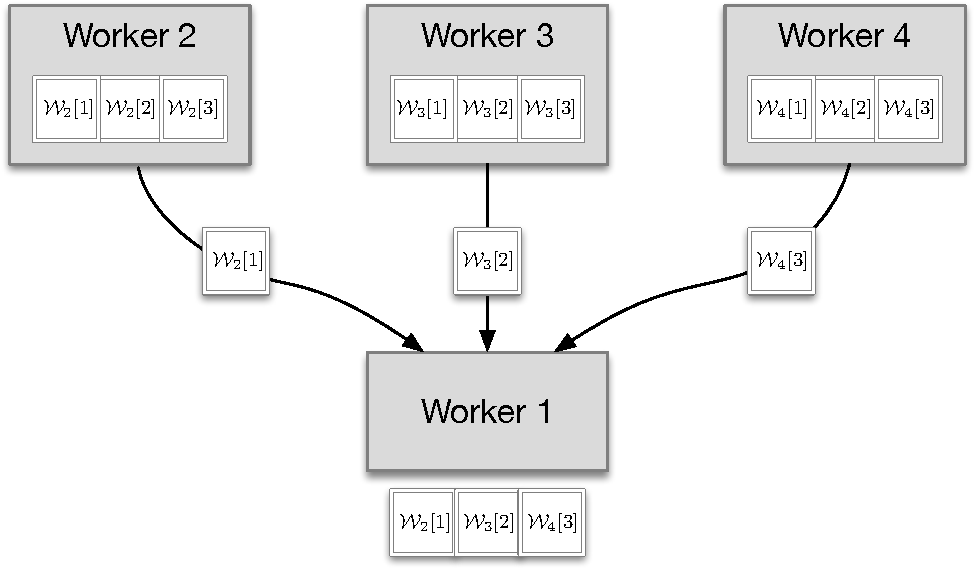
\includegraphics[width=0.3\textwidth]{pics/seg_pull.pdf}
%\caption{Segmented Pulling}
%\label{Fig: seg-pull}
%\end{figure}


\subsubsection{Model Replica}

% Like other gossip-based approaches, we use random partial aggregation as an approximation of the global aggregation. But if the number of the participating workers is too big, which could be common in a federated learning context, there might be huge deviation in such approximation if the worker aggregates local model with only one external model as there are many of them. 
% 

In traditional distributed ML scenario within the datacenter, the gossip-based solutions can choose only one other worker for aggregation but still achieve excellent convergence, because the workers ``gossip" with each other frequently such that the update of each worker are propagated through the whole network before they become too stale\cite{daily2018gossipgrad:}. However, for communication efficient FL systems, the staleness of the model updates is hard to bound as the models are trained separately for up to a few epochs. 
 

Thus as a compromise, we set a hyper-parameter \textit{Model Replica} $R$ which represents the number of the mixed model gathered by segmented pulling. To rebuild $R$ mixed models, the worker will pull $S \times R$ segments from peers. Thus increasing the value of $R$ means more segments have to be transferred through the network, which may cause bandwidth overhead. But this is necessary to accelerate the propagation and ensure the model quality. Since there is no centralized server bottleneck, the model training speed could still be faster even with extra transmission.


\subsubsection{Bandwidth-Aware Gossip Aggregation}
\begin{algorithm}[!t]

\caption{Bandwidth-Aware Combo (BACombo)}

\renewcommand{\algorithmicrequire}{\textbf{Input:}}
\renewcommand{\algorithmicensure}{\textbf{Output:}}
\SetKwFunction{SP}{{SegPulling}}
\SetKwFunction{SA}{{SegAggregation}}


\begin{algorithmic}[1]
\REQUIRE $K, T, \eta, E, \widetilde{w}_0, N, S, \epsilon $

\STATE \textbf{Each worker $i$ executes:}
\STATE $ B \leftarrow \mathbf{0} $

\FOR {$t = 0, ...,T-1$}
    \STATE $r_t \leftarrow Random()$ 
    \STATE updates ${ w}_{t}$ for $E$ epoches of SGD on $F_i$  with step size $\eta$ to obtain ${ w}_{t+1}$
    \IF{ $r_t < \epsilon $}{
        \STATE %$ \{{w}_{t,k}^\prime\}, J, \{D_j\} \leftarrow $ 
        \SP{$Random(),K, N,i$}
        \STATE update $B$ based on the \textbf{BandwidthPrediction}$(J)$}
    \ELSE {
        \STATE %$ \{{w}_{t,k}^\prime\}, J, \{D_j\} \leftarrow $ 
        \SP{$Greedy(),K, N,i$}
    } 
    \ENDIF
    \STATE $\widetilde{{w}}_{t+1} \leftarrow$ \textbf{SegAggregation} $(\{{w}_{t,k}^\prime\},{{w}}_{t+1},J ,\{D_j\})$
\ENDFOR
\item[]

\STATE \SP{$k,w_{t}$}//Run on worker $k$
{
    \STATE \quad worker $k$ updates $w_t$ for $E$ epoches of SGD on $F_k$ \\ \quad with step size $\eta$ to obtain $w_{t+1}$
\RETURN $w_{t+1}$ 
}

\item[]

\STATE \SA{$k,w_{t}$}//Run on worker $k$
{
    \STATE \quad worker $k$ updates $w_t$ for $E$ epoches of SGD on $F_k$ \\ \quad with step size $\eta$ to obtain $w_{t+1}$
\RETURN $w_{t+1}$ 
}

\end{algorithmic}	\label{BACombo} 
\end{algorithm}

            % \STATE worker selects a subset $S_{t}$ of S segments at random (each segments $s$ is chosen from  with probability $p_s$)
            
        %             \FOR {$ k = 1, ..., K$}
            
        % \ENDFOR
                % \STATE worker selects a subset $S_{t, s, r}$ of  workers at random (each worker $k$ is chosen with probability $p_k$)
%The \sys worker updates its local model using multiple "local models" from peers, each local model is a composition of model segments from different peers, we call the composition \textit{Model Replica}.

%
%the workers pull their local model to peers instead of center server.  
%
%When a worker $i$ finishes the local training and seeking to do the model aggregation, it reports its status to the index server. And then the server randomly samples a subset $K_i$ from all the participating workers as the aggregation candidates of worker $i$ and send the information about $K_i$ to worker $i$. To control the training progress, the workers of $K_i$ should have the same training iterations. When worker $i$ receives the candidate list $K_i$, it proactively fetches the model from the candidate workers, do the aggregation and then continue training on the local dataset. We use an index server to track the information of workers instead of storing peer information on the workers directly because with the growth of the workers and the variation of the network environment, the synchronization overhead can be very huge.
%
% By increasing the initiative of the workers, the bottleneck of server is removed because the communication of the server is trivial and the model parameters, which is the heavy part, are transferred among $n(n-1)$ links of all the workers.

%\subsection{Worker Segmented Transfer and Aggregation}
%After ... , the worker will ... transfer and aggregation...
% 一句话描述他们要干什么


%The idea of pulling model parameters from peers is quite similar with the Gossip-based protocols in which the workers randomly push the models to others. So they are facing the same challenge that the overall transmission quantity is increased for a single worker. In the traditional parameter server architecture, in one global iteration, the worker only has to send and receive for one time. But with the gossip methods, each worker is expected to send and receive for $|K_i|$ times in one iteration. 

%
%As shows in Figure \ref{Fig: Segment sub.1}, when the worker $i$ receives the manifest of $K_i$ candidate worker list from index server.  if the model are break in to $S$ and the replica is set to be $R$. For each segment $l$, worker $i$ selectively choose a worker $N_l$ from the candidate list, and then fetch the corresponding segment from worker $N_l$ which we denote as $\mathcal{W}[l;N_l]$. Note that this step can be parallelized, and to simplify, we use a uniform random sampling method to choose the peers. 

%With the segmented transfer method, worker $i$ receives model information from multiple peers with the transfer size equal to one model. Thus in the aggregation phase, the aggregation result can be affected by more datasets and this could help to increase the generality of the model. But if the number of the participating workers is too big, which could be common in a federated learning context, the segments can only cover few workers. Increasing the number of segments might help but an extremely small segment size could lead to over-mottled parameters. Thus as a compromise, we set a hyper-parameter $R(eplica)$ which means the number of the mixed model rebuilt by Segmented Transfer. 
%
%Another shining point of segmented transfer is privacy preserving. The complete model parameter or gradient set has the potential to leak private data information under attack. Instead of pulling the whole model from peers, \sys only collects a random subset of the parameters, which helps to preserve the data privacy. 

\begin{figure}[H]
\centering 
\subfigure[Segmented Pulling]{
\label{Fig: Segment sub.1}
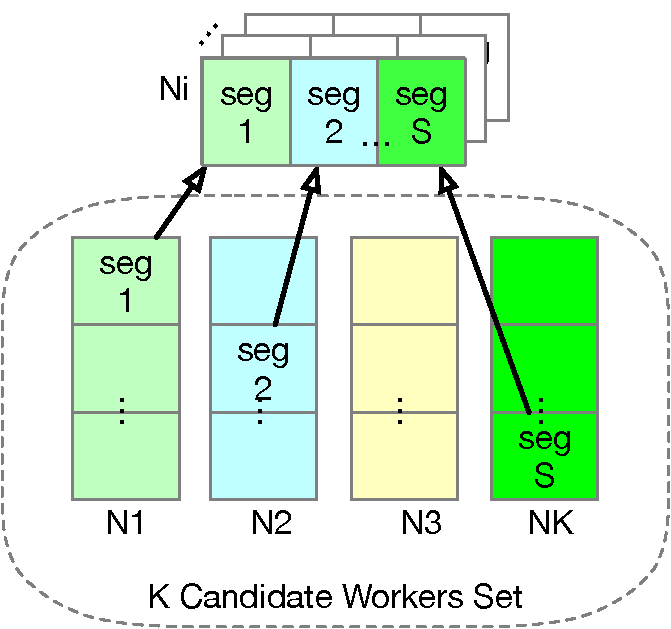
\includegraphics[width=0.2\textwidth]{pics/transfer.pdf}}
\subfigure[Segmented Aggregation]{
\label{Fig: Segment sub.2}
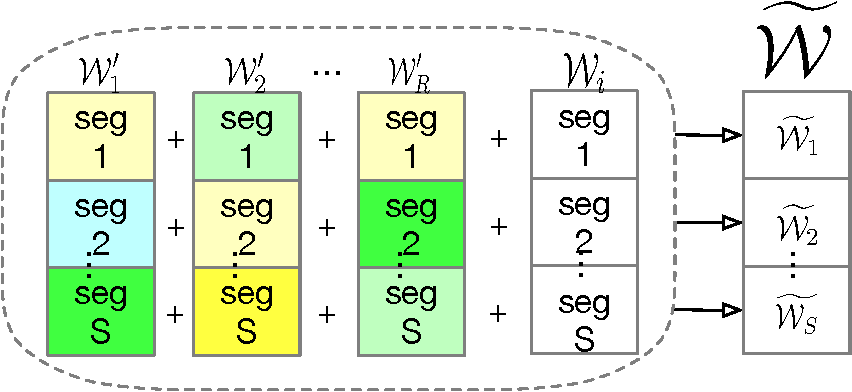
\includegraphics[width=0.225\textwidth]{pics/aggregation.pdf}}
\caption{Segmented Gossip Aggregation}
\label{Fig: Segmented schema}
\end{figure}

\subsubsection{Segmented Aggregation}
%When it fetches all the segments back, a new mixed model can be rebuilt as:
%\begin{equation}
%    \mathcal{W}^\prime = \bigcup_{l = 1}^{S} \mathcal{W}[l;N_l] \label{eq:seg_union}
%\end{equation}
Typically the model aggregation uses weighted averaging of the received model parameters with the worker's dataset size as weight. But in segmented gossip aggregation, the mixed models are patched together from different workers, so it is hard to set a reasonable weight for the mixed model as a whole. For such case, we use a segment-wise model aggregation. 

 Assume the worker $i$ has fetched all the segments and rebuilt $R$ mixed models which we represent as $\mathcal{W}^\prime_1,\mathcal{W}^\prime_2, \dots ,\mathcal{W}^\prime_R$. Then for each segment $l$, we have $R$ mixed models and one local model to aggregate. Let $P_l$ denote the set of the workers which provide the segment $l$ (worker $i$ itself is contained too) and $|D_j|$ denote the dataset size of worker $j$, then we can aggregate segment $l$ by:
 
 \begin{equation}
 \label{eq:seg_agg}
     \widetilde{\mathcal{W}}[l] = \frac{\sum_{j\in P_l}|D_j|\mathcal{W}_j[l]}{\sum_{j\in P_l}|D_j|}
 \end{equation}

Combine all the aggregated segments, and we can rebuild the final aggregation result by 
\begin{equation}
    \mathcal{W} = (\widetilde{\mathcal{W}}[1],\widetilde{\mathcal{W}}[2],\dots,\widetilde{\mathcal{W}}[S])
\end{equation}
And then the worker can continue its training until next aggregation phase comes.
 

\section{\sys Design}
In this section, we introduce \sys, a decentralized federated learning system based on segmented gossip aggregation. We firstly present the implementation details of \sys, then discuss how it handles the dynamic nature of FL workers, and finally, we give a brief analysis of the convergence of \sys.

\subsection{Implementation Details}
As a decentralized FL system, we focus on the design of the workers as the participation of the centralized server is not required during the training. However, it's important to notice that before the training starts, the server has to initialize the model parameters of each worker with the same value otherwise the training may fail to converge. 

A \sys worker follows a stateful training process as illustrated by the numbered steps in Fig.\ref{Fig: worker-arch}. At each iteration, the workers (1) update the model with local dataset and meanwhile, (2) send the segment pulling requests to other workers, once the update is finished, they (3) send the segments to the requestors as a response of the pulling requests and when all the pulling requests are satisfied, the workers (4) aggregate the model segments and start next iteration. Next, we describe the implementation details of these steps.

\noindent{\bf (1) Local Update.} The learning process starts with the worker updating the model with the local dataset. The worker takes the aggregation result of the last iteration as the input model and updates it using stochastic gradient descent(SGD) with the local data. To reduce the communication cost, the local update may contain multiple SGD rounds before the communication with other workers. We denote the communication interval or the number of SGD rounds as $\tau$, which, in typical FL systems, could be up to a few epochs.

\noindent{\bf (2) Segments Pulling.} The workers firstly decide how to partition the model. They don't have to follow the same partition rule, but for simplicity, we assume they partition the model into $S$ segments in the same way. For each segment, the worker has to select $R$ peers and sends the \emph{pulling request}, which contains a segment description and a unique identifier of the worker to indicate which part of the model is to be sent and whom it suppose to be sent to. 

Each worker has to send $S\times R$ segment pulling requests to the other workers, and \sys tries to distribute these requests evenly among all the workers to engage more links and balance the transmission workload. Thus for each request, the target worker is randomly selected from all the other workers without replacement until there is no option left, which means when $S\times R \leq n$, all the segments come from different workers. Note that for each iteration, the pulling requests can be sent even before the local update starts; in this way, the target workers can send the segments immediately when the local model is ready.

\noindent{\bf (3) Segments Sending.} The sending procedure is a twin action of the segments pulling. When the worker finishes the local update, it is ready to send its update result to others. Rather than actively pushing the model, the worker only dispatches the model segments according to the received pulling requests.

\noindent{\bf (4) Model Aggregation.} While the worker is providing the model segments to others, it is also receiving the segments it has requested previously. The model aggregation phase is blocked until all the pulling requests are satisfied, then the worker aggregates the external model segments with the local model using \eqref{eq:seg_agg} and put the aggregated segments together to rebuild the model. With the aggregation result, the worker gets back to the first step and starts the next training iteration.


\begin{figure}[H]
\centering 
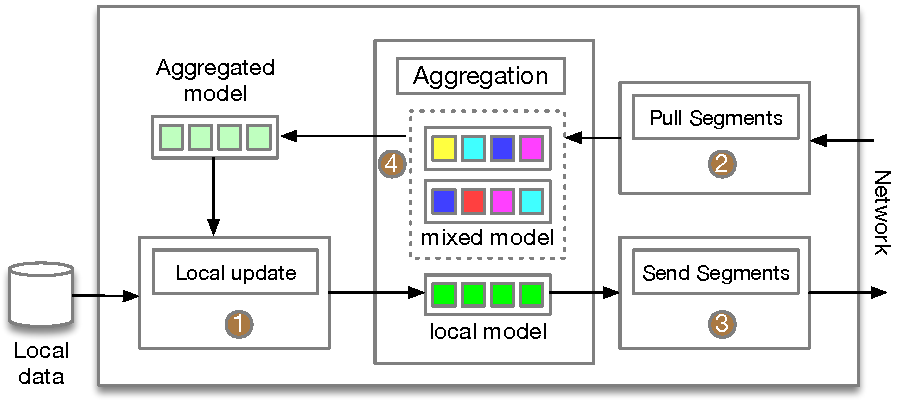
\includegraphics[width=0.49\textwidth]{pics/worker_arch.pdf}
\caption{The architecture of \sys workers}
\label{Fig: worker-arch}
\end{figure}



\subsection{Dynamic Workers}
In the context of federated learning, the participating workers are more likely to be mobile phones and embedded devices, which are often not connected to a power supply and stable network. Thus the workers in FL system are highly dynamic and unstable, and they can join and exit the federation at any time. 

Traditional distributed systems adopt the heartbeat packet and time threshold to check the status of the workers. However, these methods are not applicable with the FL system for the next two reasons: 1) The server has to maintain the heartbeat connection with all the participating workers which limits the scalability of the system. 2) The computation times of each worker vary significantly due to the difference in the computing devices and network environment.

Fortunately, the design of \sys allows us to solve this problem decently. If the worker exits accidentally, the pulling requests it sends to other workers can be canceled immediately when the target workers find it unreachable. For those workers who have requested segments from the offline worker, they can monitor the status of the target workers, and once they see the connection with the target worker is lost, they can mark it as offline, resend the request to another worker and stop pulling from the offline worker. If it is a false report due to the network fluctuation or the offline worker comes back, the offline flag can be removed as long as the communication is reestablished. 

The participation of a new worker is relatively easy to handle. When a new worker comes to the federation, it first requests a worker list either from a server or an old worker. Then it pulls the segments and aggregates them as normal only without its own local model. With the aggregation result, it can start the training with its local dataset. When it sends the pulling requests to the target workers, the target worker adds the newcomer to the worker list. Since the new worker sends the pull requests to many workers in a single iteration, its existence will be quickly noticed by all other workers, and then the new worker successfully joins the federation.




\subsection{Convergence Analysis}

\newtheorem{theorem}{\bf Theorem}
\newtheorem{define}{\bf Definition}
\newtheorem{assumption}{\bf Assumption}

Generally, the deep learning uses the gradient descent algorithms to find the model parameters that minimize a user-defined loss function which we denote it as $F(\mathcal{W})$. For the loss function, we make the following assumptions.

\begin{assumption}
{\bf (Loss function)} $F(\mathcal{W})$ is a convex function with bounded second derivative such that
\begin{equation}
    \mu \leq ||\nabla^2F(\mathcal{W})|| \leq L
\end{equation}
\end{assumption}

In a centralized learning system, the model parameters are updated with the gradient $\nabla F(\mathcal{W})$ calculated from the whole dataset. But with the federated settings, the worker $i$ updates the model with the gradient of a subset of data and we denote it as $\nabla F_i(\mathcal{W})$. To capture the divergence of these two gradients, we make the next definition.

\begin{define}
    {\bf (Gradient Divergence)} For any worker $i$ and model parameter $\mathcal{W}$, We define $\delta$ as the upper bound of the divergence between local and global gradients.
    \begin{equation}
      || \nabla F_i(\mathcal{W}) - \nabla F(\mathcal{W})|| \leq \delta
    \end{equation}
\end{define}

For a worker $i$ in our proposed system, at iteration $t$, the local model parameter $\mathcal{W}_{t,i}$ is an aggregation result of the local model and a few mixed models rebuilt from segments. As a contrast, we denote $\mathcal{W}_{t}$ as the aggregation result of all the nodes, which is the output of $FedAvg$ algorithm. Like the gradient divergence, we define aggregation divergence to measure the aggregation result.

\begin{define}
    {\bf (Aggregation Divergence)} For any worker $i$ at iteration $t$, we define $\rho$ as the upper bound of the divergence between partial and global aggregation.
    \begin{equation}
      || \mathcal{W}_{t,i} - \mathcal{W}_{t}|| \leq \rho
    \end{equation}
\end{define}

With the above assumption and definitions, we can present the convergence result of \sys. 

\begin{theorem}
\label{trm:converge}
    Let $\mathcal{W}^*$ denote the global optimum and $\mathcal{W}_0$ denote the initial model parameters, worker $i$ performs gradient descent on local dataset for $\tau$ times with learning rate $\alpha \leq \frac{1}{L}$ and then pull the segments to aggregate, the aggregation result is $\mathcal{W}_{t,i}$, the convergence upper bound of \sys is given by
    \begin{equation}
            ||\mathcal{W}_{t,i}-\mathcal{W}^*|| \leq \theta^{t\tau} ||\mathcal{W}_{0}-\mathcal{W}^*|| + (1-\theta^{t\tau})[\frac{\rho}{1-\theta^\tau} + \frac{\alpha \delta}{1-\theta}]
    \end{equation}
    where $\theta = 1-\alpha \mu$.
\end{theorem}
\newenvironment{ProofSketch}{%
  \renewcommand{\proofname}{\bf Proof Sketch}\proof}{\endproof}
  
%\begin{ProofSketch}
%This is proof
%\end{ProofSketch}

%Note that this bound is characteristic of stochastic gradient descent bounds that it converges to within a noise ball around the optimum rather than approaching it. The gap between the output and optimum comes from two part: the gradient divergence $\delta$ and the aggregation divergence $\rho$. The gradient divergence is related to the data distribution of each worker which is not alterable. According to the above inequality, the influence of $\rho$ is exacerbated when the communication interval $\tau$ increases. The aggregation divergence can be ameliorated by aggregating more models from other workers. This explains why we set a hyper-parameter $R$ to control the model replicas received from others.

Note that this bound is characteristic of stochastic gradient descent bounds that it converges to within a noise ball around the optimum rather than approaching it. The gap between the output and optimum comes from two part: the gradient divergence $\delta$ and the aggregation divergence $\rho$. The gradient divergence is related to the data distribution of each worker, which is the inherent drawback of the FL system.

According to the above inequality, the influence of $\rho$ is exacerbated when the communication interval $\tau$ increases. The aggregation divergence can be ameliorated by aggregating more models from other workers. This explains why we set a hyper-parameter $R$ to control the model replicas received from others. If we let $R=n-1$, the worker aggregates all the external models and the model divergence decreases to zero. In this situation, \sys degrades to the all-reduce scheme and has the same training result as the centralized way. However, we argue that the value of $R$ could be much smaller but still maintains the training efficiency, which is then validated in the evaluation.



















\begin{algorithm}
    \label{alg:restrict_update}
    \SetAlgoLined
    \SetKwInOut{KIn}{Input}
    \SetKwInOut{KOut}{Output}
    \caption{Restricted local update}
    \KIn{client $k$, global weights $w$, interval $\tau$}
    \KOut{local training result $w^\prime$}
    $w^\prime \leftarrow w$\;
    \For{local iteration $i=1,2,\dots, \tau$}{
        $b \leftarrow$ random batch of training samples\;
        $g \leftarrow$ the gradients of $w^\prime$ on batch $b$\;
        \eIf{$w^\prime$ is overfitted}{
            \textbf{break}\;
        }{
        $w^\prime \leftarrow w^\prime - \mu g$\;
        }
    }
    \Return $w^\prime$
\end{algorithm}

